\documentclass[submission,copyright,creativecommons]{eptcs}
\usepackage{breakurl}             % Not needed if you use pdflatex only.
\usepackage{datetime}
%\newdate{date}{04}{18}{2018}

\usepackage{graphicx} %package to manage images
\graphicspath{ {images/} }

\usepackage[rightcaption]{sidecap}
\usepackage{tcolorbox}
\usepackage{multicol}
\usepackage{float}

\usepackage{wrapfig}
\title{Blockchain methodologies applied to transaction operations on the Real Estate Market}
\author{Andres Salgado
\institute{International Technological University\\ San Jose, California, \underline{USA}}
\email{salgadoandre533@students.itu.edu}
\and
Co Authors \qquad\qquad Jorge Valdeiglesias, Kartikeya Yellayi
\institute{International Technological University\\ San Jose, California, \underline{USA}}
\email{\quad valdeiglesjorge744@students.itu.edu \quad\qquad yellayishiva1284@students.itu.edu}
}



\def\titlerunning{Blockchain principles applied to transaction operations on the Real Estate Market}
\def\authorrunning{Andres Salgado, C. Author \& Jorge Valdeiglesias, Kartikeya Yellayi}

\begin{document}
\maketitle
%\displaydate{today}
\centerline{\date{April 21 2018}}


\begin{abstract}
The blockchain concept was proposed several years ago. Only in recent years has the concept evolved into full fledged applications and frameworks that allow users to solve everyday problems with this technologies.  One of the many issues that society currently faces are the skyrocketing housing prices.  A partial reason of this increase in prices is the many intermediaries that are part of the real estate buying and selling process.  Our application attempts to find a proper way to replace some of the entities involved on the escrow process with smart contracts executed on a decentralized Ethereum network.  The paper briefly touches on historical facts related to the use and adoption of cryptocurrencies, the legal framework that is currently in place for the escrow business, and an in-depth analysis of the code base used for the test application. 
\end{abstract}

\section{Introduction}

With the advent of ``blockchain'' technologies, as well as the necessity to establish a system were transaction trust could be offloaded to machines, we ventured into exploring how a system based on the Ethereum blockchain could accurately execute a series of smart contracts in order to validate a transaction between two entities.

\section{The blockchain and its influence on crypto-currencies}

It's close to 10 years after Bitcoin was introduced by Satoshi Nakamoto. The reason crypto-currencies currently exist is due to the underlying technology made available by the blockchain. Thomas Lowenthal from Ars Technica \cite{lowenthalBitcoinEncryptedPeertopeer2011} goes onto explaining the complexities of cryptographic currencies, the concept of mining and make-work, and goes onto comparing Bitcoin against the trusty greenback which also faced hurdles when it was first put into circulation.

No currency system is perfect. One of the caveats of implementing a digital currency is the problem of double-spending.  Since there are no regulating agents (in this case governments or private entities) that can verify the authenticity of a given cryptocurrency, there has to be an engineered mechanism that can protect users from issues related to double spending and the use of counterfeit instruments. The blockchain solves these two basic problems inherent to its digital nature by applying the concepts of digital signatures and peer-to-peer networks.\cite{nakamotoBitcoinPeertoPeerElectronic}\cite{noauthor_bitcoin}.
On cppcon 2016 David Schwarz\cite{cppconCppCon2016David} at cppcon 2016 spoke about "Developing Blockchain Software".  On his talk he mentions key characteristics of "the blockchain". Section 2.1 goes onto describing such characteristics.   

\subsection{What is a blockchain and what is one good for?}
\begin{itemize}
\item Blockchains record state and history
\item State is modified by transactions
\item Everyone eventually agrees on the transactions
\item Can be used to transfer tokens and coins
\end{itemize}

Based on this list, most of us would conclude that the blockchain is merely a database, but in actuality, the blockchain -according to Schwarz\cite{cppconCppCon2016David}- manages the double-spending problem.

\subsection{What the blockchain does for bitcoin}

Figure \ref{fig:block_bloom} describes how the blockchain validates bitcoin as cryptocurrency system\cite{noauthor_bitcoin}
\begin{figure}[h]
    \centering
    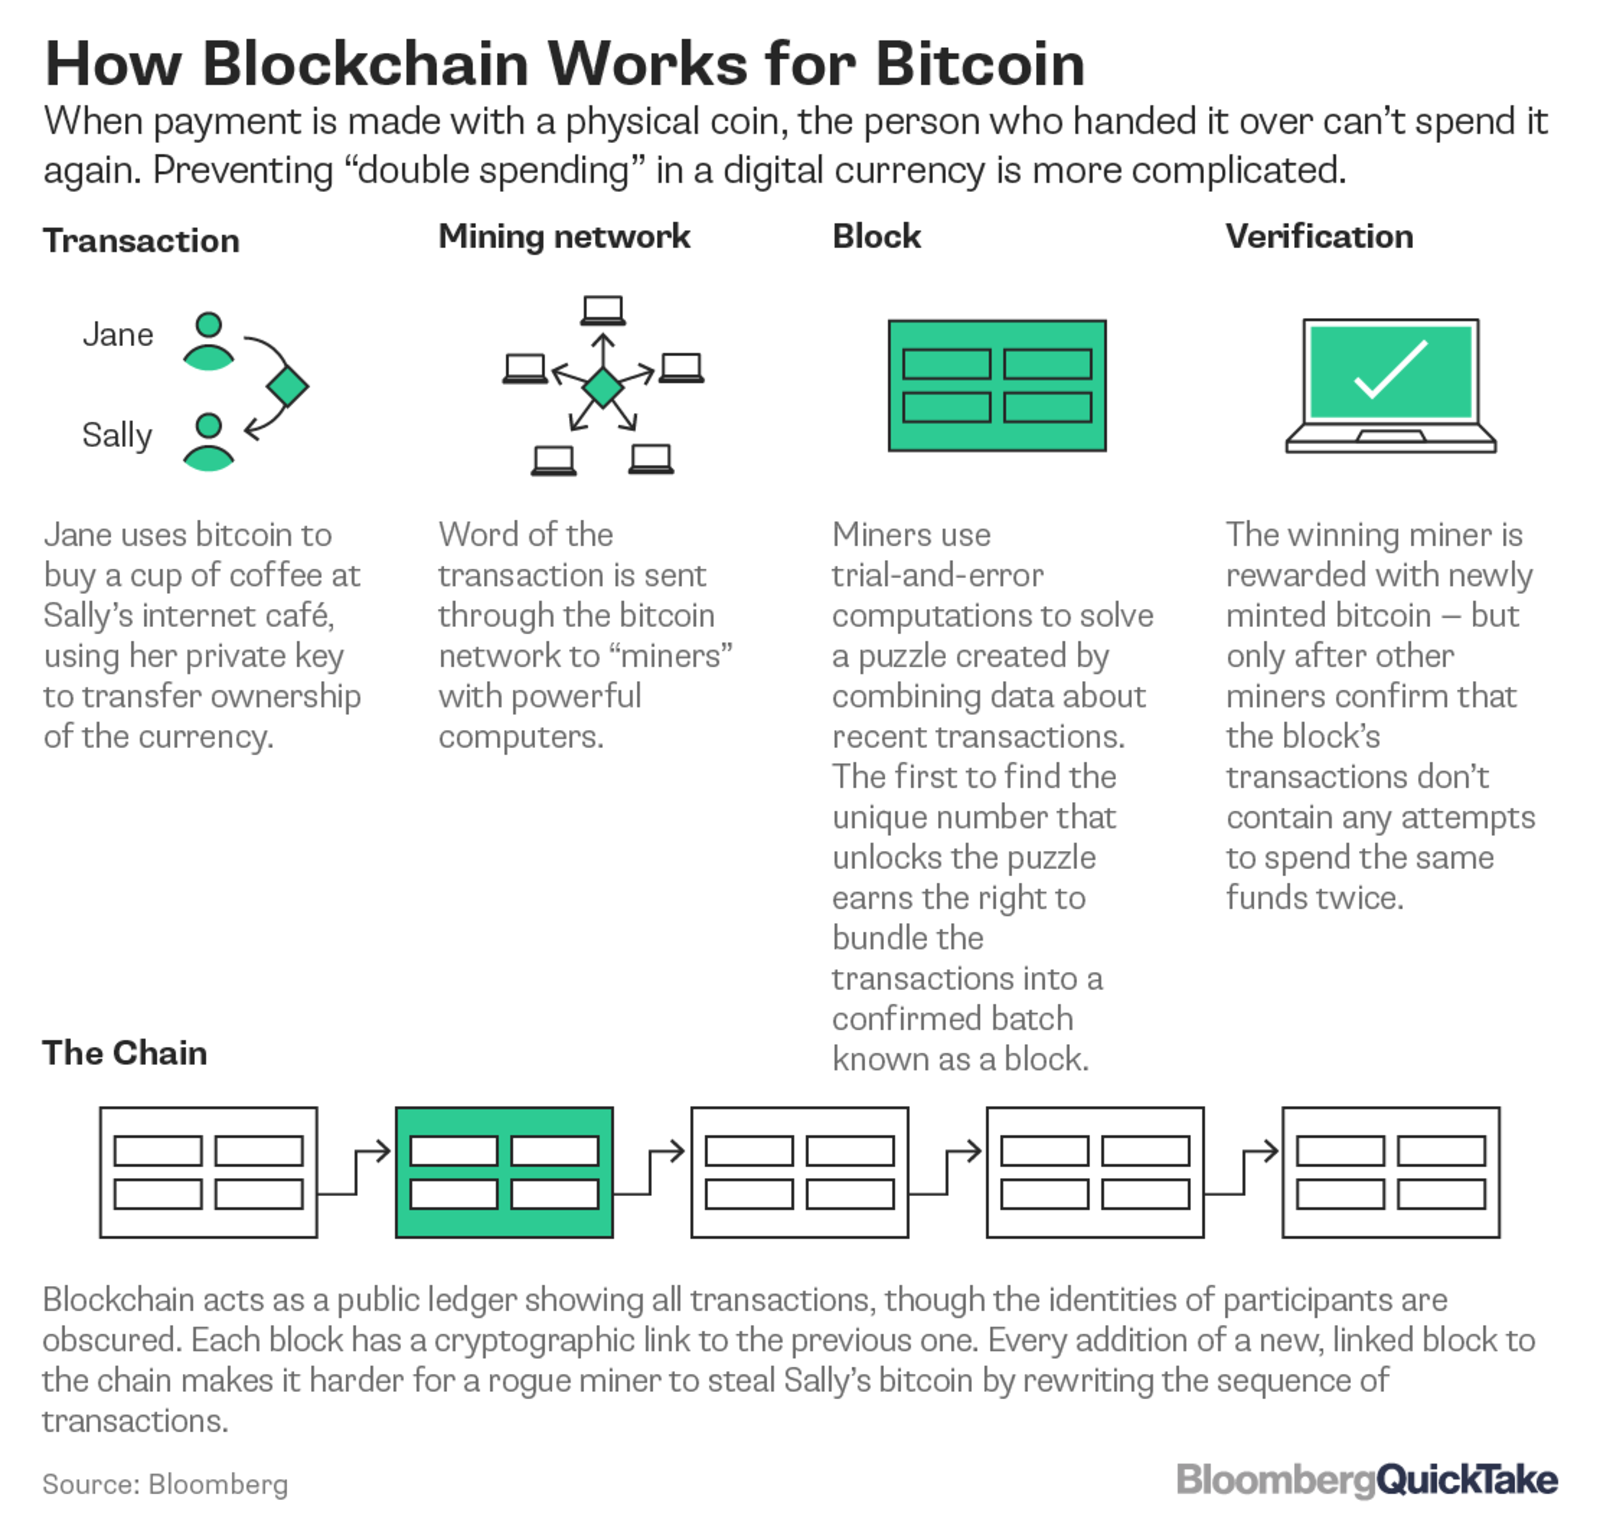
\includegraphics[width=5in]{bitcoin-blockchain-bloomberg}
     \caption{Image Source: BloombergQuicktake}
     \label{fig:block_bloom}
\end{figure}.

\subsection{Principal advantages of cryptocurrencies}
Not only does Bitcoin comply with providing security to users that require to exchange currency within the system, but by December 2017\cite{MostImportantCryptocurrencies} the 6 most important cryptocurrencies in world, among those \textit{Ethereum} which is currently the second cryptocurrency based on market capitalization \textbf{(41.4 billion)}, manage to continue on a growth path, with its value and market capitalization following an upwards trend, a sign of how confident the public feel about cryptocurrencies as a method to exchange value.

\begin{wrapfigure}{r}{0.35\textwidth}
    \centering
    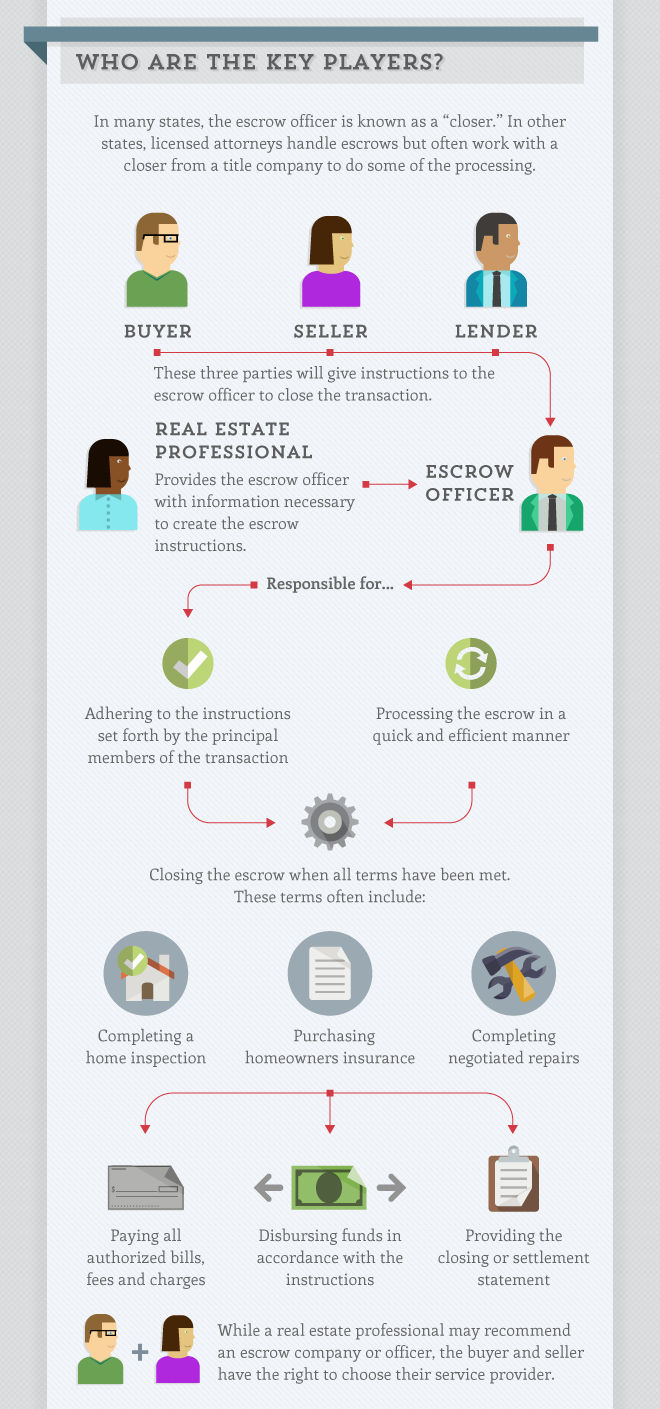
\includegraphics[width=0.30\textwidth]{infog-what-is-escrow_detail.png}
    \caption{Infographic "What is Escrow (detail)\cite{WhatEscrow} \textit{Source: First American Financial Corporation}n}
    \label{fig:info_escrow}
\end{wrapfigure}
\section{Legal Framework}
In today's current economy, a legal framework is established so that in the case that two entities require to exchange property, goods or services, this exchange can be performed with the backing of a system that effectively transfers value from one entity to another.

For the purpose of the current body of research, our model specifically targets the escrow process of a real estate sale. Figure \ref{fig:info_escrow} describes the many entities and processes involved on the execution of an escrow during the sale of a property.

\section{Beyond Bitcoin (other industries and its use)}
Besides solving the issue of how to allow for a feasible digital currency, the blockchain has opened the door towards the development of new uses of the technology, that do not necessarily address the exchange of assets in a digital manner.  This exposure has allowed millions of dollars to be poured into research and development of proper blockchain applications in a variety of fields with distinct uses and outcomes.
One of the businesses that seems to be benefiting the most from this investments is the logistics business. Many companies are involved in the process of carrying goods. Most importantly, because there are several actors involved in such process, a delay in shipment can prove to be catastrophic to huge shipments.  

Currently the majority of companies that engage in gathering data to make business decisions use different types of database systems in order to store, query and build statistical models out of collected data.  When the interaction with that data doesn't require sharing such information, companies are equipped to process it, but when two or more entities\cite{BlockchainGoesCryptoCurrency2016} need to share such data, it is often complicated to achieve a consensus on how such exchange should be handled.\footnote{Olga Kharif on her article "Blockchain Goes Beyond Crypto-Currency" explains how companies in Finland, Sweden, Estonia and Latvia are beginning to use a blockchain system in order to share information.}

\section{Ethereum and smart contracts}
Back in 1996, Nick Szabo\footnote{Nick Szabo is credited as one of the first proponents of the us of smart contracts on the digital realm.} layed much of the ground work of what we currently know as \textit{"Smart Contracts"}.  On \textit{"Smart Contracts: Building Blocks for Digital Markets"}\cite{NickSzaboSmart} Szabo makes a conspicuous argument on how our society has built a structure based on the common law of contracts.  He\footnote{Szabo does a marvelous job on explaining how our society arrived to the use of contracts and how these contracts are the bedrock of a free market economy.} is meticulous when explaining the role that contracts play into our current free market economy.  The article's introduction does not try to impose digital contracts as a replacement to our current system of values and the concept of agreements and contracts, but instead opens the door to a discourse on how computers in a digital society can improve or aid towards making the then current system more functional.

Experts conclude that \textit{Bitcoin} has done to the blockchain what e-mail did to the internet.  To further this notion of what the blockchain is capable of, it can be said that \textit{Bitcoin} is a digital currency using the blockchain as a vehicle to function digitally.  There are certain tasks that \textit{Bitcoin} can perform, but they are limited compared to that of the scope of what \textit{Ethereum} does.  One of the main advantages of \textit{Ethereum} is that it applies the same principles that the blockchain uses on \textit{Bitcoin} with the added functionality of smart contracts\footnote{Smart contracts are currently handled by the Solidity language.  Further information about solidity can be found at the development website \url{https://solidity.readthedocs.io/en/develop/}\cite{SoliditySolidity23}} as a method to exchange any item of value, this being money, content, shares or property.

Due to the advantages that \textit{Ethereum} offers, it was chosen to dig deeper into finding a toolset that would allow the app to thrive towards developing a self-serving real estate property exchange tool.

\subsection{RSA silently working on the background}
Szabo puts great emphasis on explaining the background of RSA\cite{milanov2009rsa} and its critical role on smart contracts.  The ideal metaphor uses two subjects -in this case Alice and Bob- to explain how public cryptography's mathematical intricacies work to create a pair of \textit{keys} in this case a public one and private one that serve as a cryptography based exchange of messages.  The importance of the use of RSA based encryption is directly related to the underpinning of the principles of contract design\footnote{Szabo goes on to explaining these principles on the \textit{Some Basic Principles of Contract Design} subsection of \cite{NickSzaboSmart}} and are rooted on common law, economic theory, and contractual conditions, which in turn derive the principles of observability, verifiability, privity, and enforceability.

\subsection{Smart Contract definition}
An abridged definition of the smart contract provided by the \textit{Solidity} documentation page goes as follows:
\begin{quote}
    \textit{A contract in the sense of Solidity is a collection of code (its functions) and data (its state) that resides at a specific address on the Ethereum blockchain.\cite{IntroductionSmartContracts}}
\end{quote}
In a strict technical sense, the smart contract is programmable to comply with any set of defined conditions.  Because the smart contract is rooted in code, any prerequisite that was celebrated between two parties on a traditional contract, can have its clauses translated into code, therefore allowing for any legal conditions to exist digitally.

Figure 3 llustrates how a smart contract would execute the sale of a property.  In this case two parties, the buyer and the seller, \textbf{exchange} an asset through a contract that supports the digitizing of a land deed and the subsequent digitizing of the currency, allowing for an ordered settlement and thus cementing the idea that the ownership of the asset was properly transferred to the new owner\cite{WhatAreSmart}.
\begin{figure}
    \centering
    \label{fig:howsmartcontractsworks}
    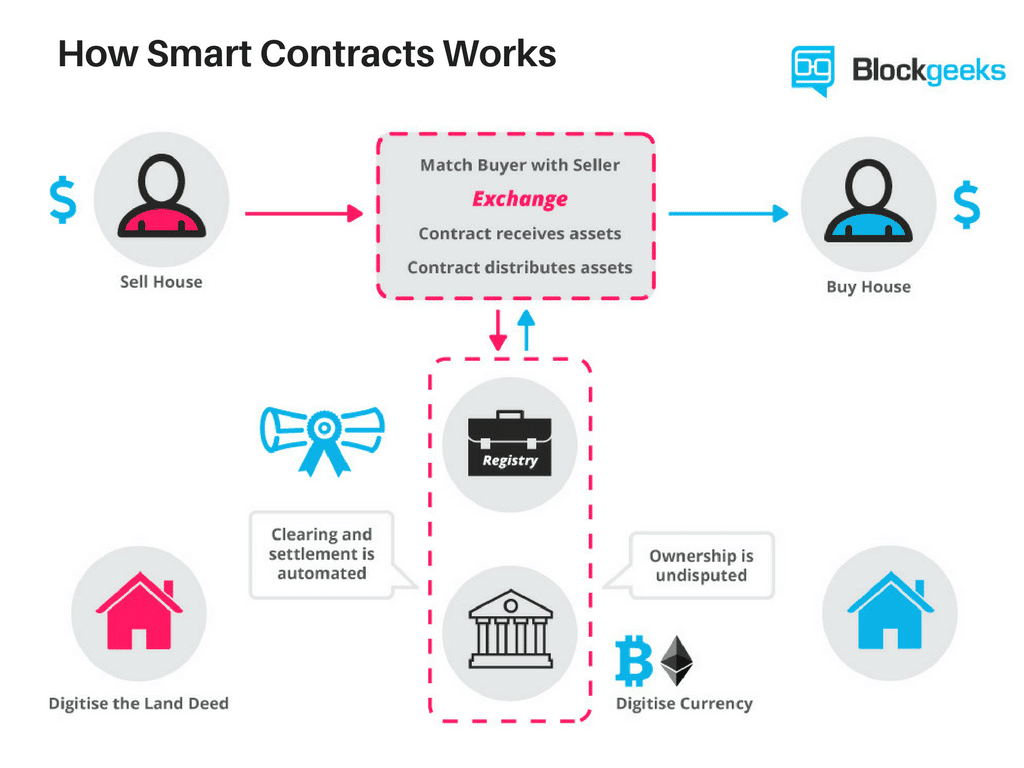
\includegraphics[width=5in]{How-Smart-Contracts-Works-1.png}
     \caption{Image Source: Blockgeeks}
\end{figure}

\subsection{Zeroing on Ethereum}
\textit{Ethereum's} versatility, served as the perfect platform to deploy a generalized decentralized app seeking to solve smart contract transactions.  Dr. Gavin Wood in his introduction to \textit{ETHEREUM: A SECURE DECENTRALISED GENERALISED TRANSACTION LEDGER} summarizes the objectives of building \textit{"a trustful object messaging compute framework."}\cite{wood2014ethereum}Parting from these principles the platform choice selected for accomplishing the objective of the thesis  revolved around the use of a framework grounded on \textit{Ethereum}. 

Research concluded that the chosen framework needed to have current front-end and back-end technologies, as well as to show signs of current community engagement and active development.  
\begin{multicols}{2}
[
\section{Truffle as a development platform}
\textit{Truffle} is a Javascript based development framework\cite{TruffleDocumentation}. \textit{Truffle} offers the following advantages as a tool:
]
\begin{itemize}
    \item Built-in smart contract compilation, linking, deployment and binary management.
    \item Automated contract testing for rapid development.
    \item Scriptable, extensible deployment and migrations framework.
    \item Network management for deploying to any number of public and private networks.
    \item Package management with EthPM and NPM, using the ERC190 standard.
    \item Configurable build pipeline with support for tight integration.
    \item External script runner that executes scripts within a Truffle environment.
\end{itemize}
\end{multicols}

\begin{multicols}{2}
[
\section{Application requirements (what to install)}
The following software is required to run the experimental app:
]
\begin{itemize}
\item Truffle
\item Ganache
\item Node.js
\item MongoDB
\item Metamask
\item Compatible Browser (Google Chrome or any other browser that supports the Metamask extension)
\item Docker
\end{itemize}
\end{multicols}

\subsection{Ganache}
In order to deploy and test the validity and accuracy of contracts written within the coding environment, it is necessary to write the contracts to the blockchain.  The creators of \textit{Truffle} simultaneously develop and maintain a separate component named \textit{Ganache}.  \textit{Ganache}\cite{Ganache} is a personal deployable test Ethereum network capable of accepting commands, with a GUI interface that allows users to inspect and control how the chain operates.  It is a requirement for Ganache to run in the background in order to properly test the validity and actionability of any given contract code executed within the application.

\section{Application logic}
Property state depicts the logic around the contract and how its state changes based on data input and user interaction.
\begin{figure}[h]
    \centering
    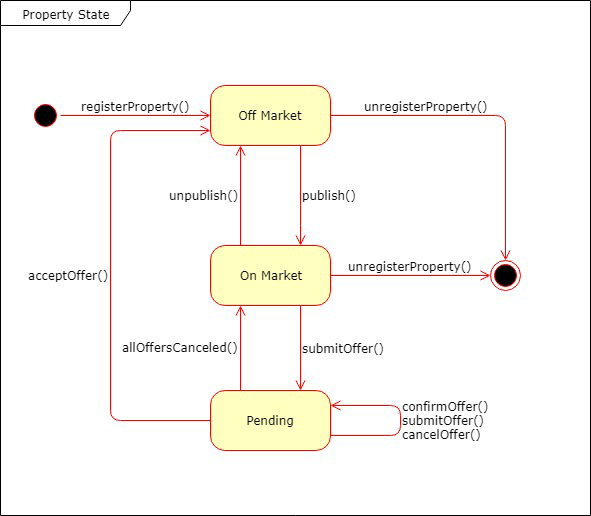
\includegraphics[width=5in]{property_state_uml.png}
    \label{fig:property_state_uml}
    \caption{Property State Diagram. Author: Jorge Valdeiglesias}
\end{figure}

\begin{multicols}{2}
[
\section{Application usage scenarios}
On the current development stage the following changes of state are supported:
]
\begin{itemize}
\item Contract deployment
\item Token transfer
\item Property publishing
\item Offer submission
\item Party acceptance
\end{itemize}
\end{multicols}


\subsection{Contract Deployment}
The contract deployment stage is intimately related to the correct execution of the \textit{Truffle} environment.  The following requirements should be satisfied prior to running the commands shown in \textit{Figure 3}
\begin{itemize}
\item Windows, Linux or Mac OS X
\item NodeJS 5.0+ recommended.
\end{itemize}

\begin{figure}[h]
\begin{tcolorbox}
%\begin{align}
\begin{verbatim}
npm install -g truffle
\end{verbatim}
%\end{align}
\end{tcolorbox}
\caption{npm command}
\end{figure}

After this step it is required before any new \textit{truffle} operation, to have a functioning test blockchain in place.  \textit{Ganache} is the tool of choice.  It is availaible in two flavors, a desktop application and a command-line tool.  For current test purposes the user will download the appropriate desktop application compatible with their running operating system. 

Figure 6 shows an account overview after successful \textit{Ganache} installation.\footnote{An extensive guide on how to install and deploy \textit{Ganache} is available at the following address \url{http://truffleframework.com/docs/ganache/using}}
\begin{figure}[h]
    \centering
    \label{fig:ganache_dashboard}
    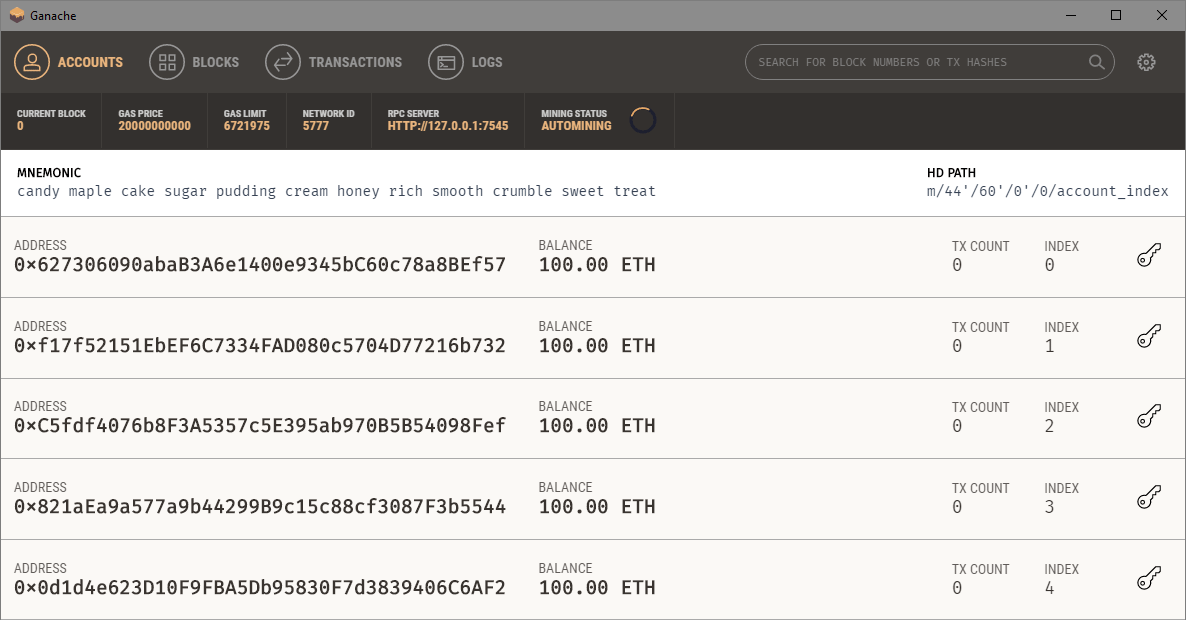
\includegraphics[width=5in]{ganache_accounts.png}
     \caption{Image Source: CONSENSYS 2017}
\end{figure}.

\subsection{Token transfer}
The token transfer stage is a practical step that shows an actual transaction between two parties taking place.  Digital assets are transferred between two key holders.  The underlying code for this operation is driven by the \textit{solidity} framework. Figure \ref{fig:token_transfer_code} shows the code involved during this stage.

\begin{figure}[h]
\begin{tcolorbox}
\begin{verbatim}
  function transfer(address _to, uint256 _value) public returns (bool) {
    require(_to != address(0));
    require(_value <= balances[msg.sender]);

    balances[msg.sender] = balances[msg.sender].sub(_value);
    balances[_to] = balances[_to].add(_value);
    emit Transfer(msg.sender, _to, _value);
    return true;
  }
\end{verbatim}
\end{tcolorbox}
\caption{Token transfer function based on \textit{OpenZeppelin}\cite{ZeppelinsolidityOpenZeppelinFramework2018}}
\label{fig:token_transfer_code}
\end{figure}

\subsection{Property Publishing}
Property publishing is one of the core features of the researched app. This feature allows a platform user to add a listing of a property, which in turn initiates a transaction that gets recorded on the blockchain.  This step would be akin to having a seller start the escrow process during a regular sale on the real estate market. Figure \ref{fig:property_publishing_code} shows the code involved during this stage.
\begin{figure}[h]
\begin{tcolorbox}
\begin{verbatim}
    function registerProperty(string propertyId, uint256 propertyPrice)
    public {
        properties[propertyId].owner = msg.sender;
        properties[propertyId].price = propertyPrice;
        properties[propertyId].state = 0;
        emit PropertyUpdated(propertyId, msg.sender);
    }
\end{verbatim}
\end{tcolorbox}
\caption{State change once property is registered}
\label{fig:property_publishing_code}
\end{figure}

\subsection{Offer submission}
On this stage the smart contract updated the state of the \textit{submitOffer} function based on the user input on the value of the property.  This action triggers a series of events including notifying the intended seller of the buyers established offer.  Figure \ref{fig:offer_submission_code} contains the code used for satisfying this function.
\begin{figure}[h]
\begin{tcolorbox}
\begin{verbatim}
    function submitOffer(string propertyId, uint256 offer) public
    onlyOnMarket(propertyId) {
        balances[msg.sender] -= offer;
        offers[msg.sender].propertyId = propertyId;
        offers[msg.sender].offer = offer;
        offers[msg.sender].submittedAtBlockNumber = block.number;
        properties[propertyId].state = 2;
        emit PropertyUpdated(propertyId, msg.sender);
    }
\end{verbatim}
\end{tcolorbox}
\caption{State change once property is registered}
\label{fig:offer_submission_code}
\end{figure}

\section{Conclusions}
Blockchain technologies are evolving at an accelerated pace. The application presented on this paper tackles an issue at the heart of the Real Estate market.  If this application was to be deployed into production, it would replace a significant number of job posts directly related to the escrow business.  

The authors are cautiously optimistic that in order for the free market to start accepting the use of applications and services dependent on the blockchain, a series of processes need to be put in motion.  The most important movement towards cryptocurrency adoption has already began to cause ripples on financial markets.  It is only a matter of time until goods and services exchanged on the blockchain based currency markets begin to displace those traded via fiat currencies, and at the current pace of innovation, it is apparent that there is willingness from venture capitalist to properly fund companies interested in developing solutions based on a generalized global ledger. 

We are anticipating an upward trend in interest towards the use of blockchain technologies, and predict that based on successful deployment of decentralized applications, the industry will create a snowball effect that most likely will disrupt the value exchange mechanisms currently in place globally. 

\subsection{Project tangible achievements}
The application proposed on this paper achieves the following objectives:
\begin{itemize}
    \item Successfully establishes a private local Ethereum test blockchain.
    \item Allows for proper user authentication via private keys in order to affect the blockchain transaction sequence.
    \item Successfully records a token transfer transaction between \textit{User A} and \textit{User B}.
    \item Allows for \textit{User A or B} to publish a property for sale.  The publishing of the property gets recorded on the blockchain as well.
    \item Establishes the validity of the smart contract code written on every change of the property state figure (as seen on Figure 4).
    \item Enables the exchange of value, albeit a fictitious one, between seller and buyer within the ethereum based test environment.
    \item Defines a proper implementation of the application on Web 3.0 environment.
\end{itemize}

\section{Acknowledgements}
We would like to thank Dr. Alex Wu for his invaluable input during the course of our studies and research

\newpage
\bibliographystyle{acm}
\begin{multicols}{2}
\bibliography{biblio}
\end{multicols}
\end{document}
